Information retrieval (IR) is the task of finding {\it relevant} documents from a large collection of texts to fulfill a user's information need, typically expressed in the form of a textual query~\cite{singhal2001modern}.
The notion of relevance from the user's perspective (i.e., {\it intent}) can be amorphous~\cite{8160827}, and a query alone may not fully capture user information needs~\cite{ruthven_lalmas_2003,Taylor1962ThePO}.
\begin{figure}[t!]
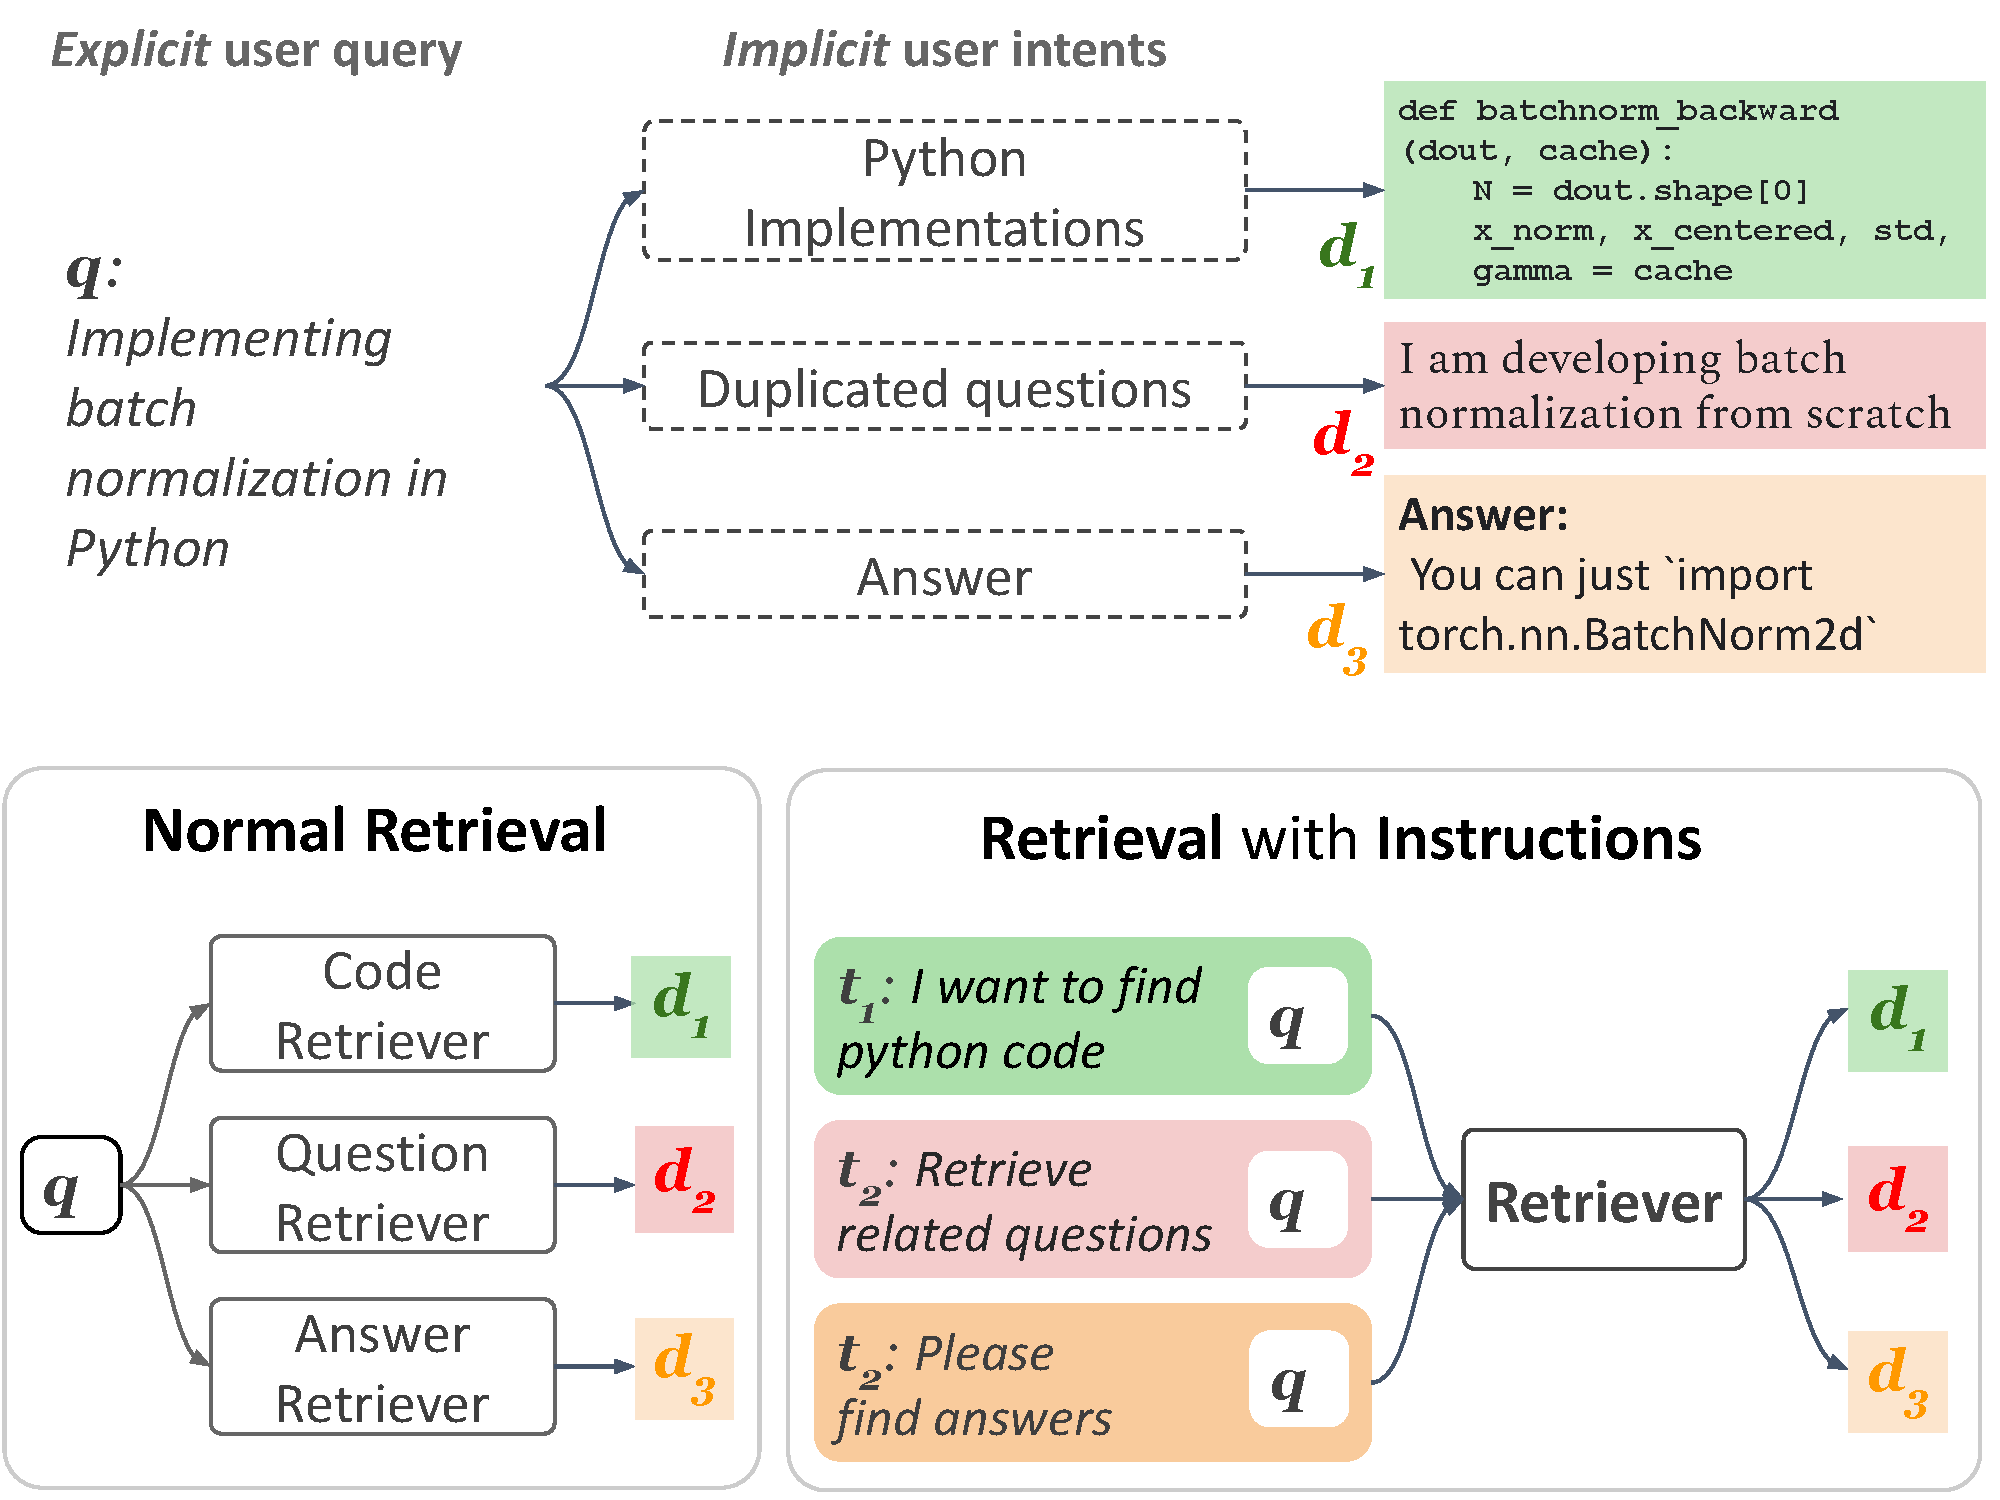
\includegraphics[width=8cm]{imgs/teaser_v7.pdf}\caption{
User intents are not fully captured in query $\boldsymbol{q}$ only (top). 
Conventional approaches (bottom left) take a query and retrieve documents from a closed corpus using a task-specific retriever. 
\emph{Retrieval with instructions} (bottom right) takes a query and explicit intent and retrieves documents aligning with the user's expectations.
} \label{fig:teaser}
\end{figure}
As illustrated in Figure~\ref{fig:teaser} (top), given the same query, ``\textit{implementing batch normalization in Python},'' a user may want to retrieve a passage that describes how to do the task or to identify a similar query, or even to directly locate a code snippet.

Most existing work tries to learn those {\it implicit} intents from labeled data (e.g., pairs of queries and relevant documents), yielding separate models for different intents 
as shown in the bottom left of  Figure~\ref{fig:teaser}. 
This approach has several limitations. 
First, a vast number of annotated examples may be required to train a model to capture the task-specific notion of relevance, while they could benefit from the abundance of data available from related tasks.
Second, a model trained on one task may not easily transfer to new tasks that are not closely related. 

In this work we advocate for a new task formulation, \textit{retrieval with instructions}, to {\it explicitly} model a user's search intent {by providing a natural language description of the search task (i.e., an instruction). }
Here, the goal of retrieval systems is to retrieve documents that are both relevant to the query \emph{and} well-suited to the instructions.

{
Despite active research in other settings, instruction-following has not been systematically explored in retrieval, partly due to the lack of annotated resources.
}
To facilitate research in retrieval with instructions, we introduce \rib ({\bf B}ank of {\bf E}xplicit {\bf R}et{\bf R}ieval {\bf I}nstructions), a collection of approximately 40 retrieval datasets with diverse instructions in a unified format{, covering 10 diverse domains. }
{Each task has on average 3.5 diverse instructions annotated by experts, following our novel instruction schema for retrieval tasks.}

{
{
We use \rib to train \model (\textbf{T}ask-\textbf{a}ware \textbf{R}e\textbf{T}riever), a single multi-task retrieval system 
% \model is a task-aware retrieval system, i.e., a system 
that follows instructions to perform diverse tasks with no parameter updates on each task. 
% \model is able to adapt to new retrieval tasks with no parameter updates. 
}}
We employ two widely explored architectures: 
\model-dual is a dense dual-encoder architecture, retrieving documents based on the similarity of independently encoded query and document embeddings; \model-full calculates probabilities of a document being relevant to the query according to the instruction using a cross-encoder. 
\model is trained with carefully designed negative samples, including our novel {instruction-unfollowing negatives samples}.

The \model models, particularly \model-full yields state-of-the-art results on two popular zero-shot retrieval benchmarks, BEIR~\cite{thakur2021beir} and LOTTE-pooled~\cite{santhanam-etal-2022-colbertv2}, outperforming systems using three times more parameters (\citealt{nogueira-etal-2020-document, ni2021large, muennighoff2022sgpt}) as well as task-specific retrievers trained on millions of automatically generated examples~\cite{promptagator,wang-etal-2022-gpl}.

We further introduce a new evaluation setup, \task ({\bf Cross}-task {\bf Cross}-domain Retrieval), where a system needs to handle queries with diverse intents to find relevant documents from a large-scale, cross-domain pooled corpus{, simulating challenges in real-world retrieval applications.}
In this under-explored setting, \model outperforms other state-of-the-art methods, demonstrating its ability to find documents in a large-scale open-domain corpus by leveraging explicit textual intents. 
Our analysis shows that training a model on diverse tasks with instructions, {our new negative samples leveraging instructions} and giving informative instructions are crucial.

In summary, our contributions are as follows: 
\vspace{-0.1cm}
\begin{itemize}
\itemsep-0.2em 
\item \emph{Retrieval with instructions}, a new formulation to model users' intent {\it explicitly}
% that reduces query ambiguity using explicit instructions
(Section~\ref{sec:task_formulation}). 
\item {\rib, a new large-scale collection of approximately 40 retrieval datasets in diverse domains with instructions (Section~\ref{sec:dataaset}). }
% \akari{highlight instruction scheme for retrieval tasks }
\item {\model, a task-aware retriever trained on \rib that advances state of the art on zero-shot and cross-task retrieval (Section~\ref{sec:method})}. 
\end{itemize}
